%        1         2         3         4         5         6         7         8

\documentclass[letterpaper,10pt,conference]{ieeeconf}



\IEEEoverridecommandlockouts

\overrideIEEEmargins



\usepackage[caption=false,font=footnotesize]{subfig}

\usepackage{graphicx}

\usepackage{booktabs}

\usepackage{array}

\usepackage{algorithm}

\usepackage{algpseudocode}

\usepackage{amsmath}

\usepackage{amssymb}

\usepackage{cite}

\usepackage{xurl}



\makeatletter

\let\NAT@parse\undefined

\makeatother

\usepackage[
    colorlinks=true,
    citecolor=blue,
    linkcolor=blue,
    urlcolor=blue
]{hyperref}



\title{\LARGE \bf
A Structured LLM-Assisted Decision Pipeline for Unsignalised Intersection Control in SUMO
}



\author{Cheng Peng}



\begin{document}
\begin{titlepage}
    \begin{center}
        \vspace*{1cm}
        {\huge A Structured LLM-Assisted Decision Pipeline for Unsignalised Intersection Control in SUMO}
        \vspace{0.5cm}

        {\large By}

        \vspace{0.5cm}
        \textbf{PENG, CHENG}
        \vspace{1.5cm}

        {\huge\textbf{MSc Robotics Dissertation}}

        \vspace{10mm}
        
\includegraphics[scale=0.6]{logos/bristolcrest_colour.pdf}
        \hspace{5mm}
        
\includegraphics[scale=0.35]{logos/UWE_insignia.png}

        \vspace{10mm}
        {\large School of Engineering Mathematics and Technology\\
        \textsc{University of Bristol}}\par

        \vspace{0.2cm}

        \&\par

        \vspace{0.2cm}

        {\large School of Engineering\\
        \textsc{University of the West of England}}\par

        \vspace{0.8cm}
        \begin{minipage}{10cm}
        \centering
        A MSc dissertation submitted to the University of Bristol and the University of the West of England in accordance with the requirements of the degree of \textsc{Master of Science in Robotics} in the Faculty of Engineering.
        \end{minipage}\par
        \vspace{0.8cm}
        \today
    \end{center}

    \vspace{1cm}
    {\large{Declaration of own work}}

    I declare that the work in this MSc dissertation was carried out in accordance with the requirements of  the University\'s Regulations and Code of Practice for Research Degree Programmes and that it  has not been submitted for any other academic award. Except where indicated by specific  reference in the text, the work is the candidate\'s own work. Work done in collaboration with, or with the assistance of, others, is indicated as such. Any views expressed in the dissertation are those of the author.

    \begin{flushright}
    Name and Date
    \end{flushright}

    \vspace{1cm}
    {\large{Ethics statement}}

    \textit{To fill in according to the Dissertation Handbook Section 3.2.}

    \begin{flushright}
    Name and Date
    \end{flushright}
\end{titlepage}

\maketitle
\thispagestyle{empty}
\pagestyle{empty}

\begin{abstract}

Large language models (LLMs) offer flexible high-level reasoning for autonomous systems, but their contribution is difficult to identify when deterministic fallback, validation, and safety mechanisms can also determine the executed action. This dissertation develops a structured LLM-assisted decision pipeline for unsignalised intersection control in SUMO and evaluates both complete-system performance and model-specific contribution. Phase~1 compared Rule-Based, Raw LLM, Hybrid, and Hybrid + Safety pipelines over 24 formal 4V and 8V runs. The fallback-capable LLM-assisted pipelines achieved lower operational waiting and higher mean speed than the selected Rule-Based baseline, but fallback dominated provider operation, so the advantage could not be attributed independently to successful live-LLM reasoning. Phase~2 addressed this limitation by constraining planning to deterministic safe candidate groups and comparing a Gemini candidate selector with a strong deterministic cooperative comparator in 36 valid matched closed-loop runs. Across 93 Gemini decisions, 89 matched the comparator, four were identifiable legal disagreements, and no fallback occurred. The repeated S3 12V disagreement involved Gemini selecting smaller legal groups and was associated with less efficient descriptive outcomes in that condition; no general Gemini traffic-performance advantage was demonstrated. All formal Phase~2 episodes were collision-free, although no safety-verifier intervention was observed. Synchronous Gemini latency remained high and variable, limiting practical deployment. The principal contribution is an attribution-aware and deterministic-safety-constrained method that separates provider reliability, parsing, fallback, candidate feasibility, planner choice, safety intervention, and closed-loop traffic consequence when evaluating LLM-assisted autonomous decision pipelines.

\end{abstract}



\section{Introduction}



Unsignalised intersections are a compact but challenging example of cooperative decision making in autonomous transportation. Multiple vehicles may approach a shared conflict region simultaneously, and each vehicle must determine whether to proceed, wait, or yield while accounting for the intentions and movements of others. A controller that is overly conservative can maintain conflict avoidance at the cost of unnecessary waiting and low traffic efficiency, whereas an overly permissive controller can increase the risk of incompatible movements. Effective intersection management therefore requires a balance between efficiency, coordination, and safety.



Traditional approaches to autonomous intersection management generally rely on predefined traffic rules, reservation mechanisms, optimisation, or explicit cooperative policies \cite{Dresner2008,Safarov2022,Zhao2025}. These approaches provide deterministic and interpretable behaviour, but their decisions are typically constrained by assumptions encoded during system design. As traffic interactions become more context dependent, this motivates investigation into decision mechanisms that can reason over structured descriptions of the current traffic state rather than relying exclusively on a fixed set of handcrafted rules.



Large language models (LLMs) provide one possible mechanism for such context-sensitive reasoning. Recent work has demonstrated the use of language models for planning, embodied reasoning, and decision support in autonomous systems \cite{Huang2022,Driess2023,Wen2023,Jin2023,Cui2024,Yang2024,Hou2025,Li2024}. In principle, an LLM can receive a structured representation of an intersection state and produce high-level actions for multiple vehicles. This makes LLMs attractive as a flexible reasoning component within a modular traffic-control pipeline.



However, integrating an LLM into a safety-relevant control system introduces an important evaluation problem. A practical LLM-assisted controller cannot normally rely on the model alone. Provider requests may fail or experience high latency, generated responses may violate the required output format, and model decisions may require deterministic validation before execution. Consequently, an operational pipeline may also contain parsing, fallback policies, cooperative post-processing, and safety verification. These components improve robustness, but they make the source of observed performance difficult to identify. If an LLM-assisted pipeline outperforms a conventional baseline, the improvement may originate from successful model reasoning, deterministic fallback behaviour, downstream processing, or a combination of these mechanisms.



This distinction between \emph{pipeline-level performance} and \emph{model-level attribution} motivates the present study. Rather than asking only whether an LLM can be connected to a traffic simulator, this work investigates whether an LLM-assisted cooperative control pipeline can improve simulated intersection performance and whether any observed improvement can be attributed to the live language model itself. This requires evaluation at both the traffic level and the internal decision-pipeline level. Traffic metrics describe the behaviour of the complete controller, whereas provider diagnostics, fallback records, and decision provenance are required to determine which component actually produced the executed actions.



To investigate this problem, a modular control framework is implemented using the SUMO microscopic traffic simulator. The framework separates state representation, LLM interaction, structured-output parsing, deterministic fallback, cooperative processing, safety verification, and final action execution. The investigation proceeds in two connected phases. Phase~1 evaluates complete controller pipelines and establishes the attribution problem created by provider failure, deterministic fallback, and limited behavioural discrimination. Phase~2 is a research refinement motivated by those findings: it retains the structured pipeline and deterministic safety authority while comparing a Gemini candidate selector with a strong deterministic cooperative comparator over identical safe candidate groups in matched closed-loop episodes.



The study addresses the following research questions:



\begin{itemize}

    \item \textbf{RQ1:} How do the evaluated fallback-capable LLM-assisted controller pipelines compare with a standalone rule-based controller in traffic efficiency and completion, and to what extent can their behaviour be attributed to the live LLM?

    \item \textbf{RQ2:} When provided with identical privacy-minimised local state and deterministic safe candidate passage groups, how does Gemini candidate selection compare with a deterministic cooperative comparator in decision agreement and closed-loop traffic outcomes?

    \item \textbf{RQ3:} How does deterministic safety verification constrain final vehicle actions, and what safety-verifier interventions and collision outcomes are observed in the evaluated scenarios?

    \item \textbf{RQ4:} How do planner decisions and closed-loop outcomes vary across the evaluated mixed-turn interaction scenarios and bounded 8V, 12V, and 16V traffic scales?

\end{itemize}



The objectives of the study are:

\begin{itemize}

    \item \textbf{O1:} Develop a modular LLM-assisted intersection-control pipeline with explicit fallback, cooperative processing, safety verification, and decision provenance.

    \item \textbf{O2:} Compare complete LLM-assisted pipelines with a standalone Rule-Based controller while distinguishing pipeline performance from model attribution.

    \item \textbf{O3:} Construct a privacy-minimised deterministic safety envelope for mixed-turn LLM planning using route semantics, compatible candidate groups, validated model output, and controlled execution.

    \item \textbf{O4:} Compare Gemini fairly with a strong deterministic cooperative comparator over identical state and safe candidates using independent matched closed-loop episodes.

    \item \textbf{O5:} Evaluate decision agreement, closed-loop traffic outcomes, provider and parser reliability, fallback behaviour, safety observations, latency, and bounded scenario and scale behaviour.

\end{itemize}



Phase~1 first compares complete fallback-capable LLM-assisted pipelines with the standalone Rule-Based controller. Its provider, fallback, and provenance evidence reveals that favourable pipeline outcomes do not by themselves identify a live-LLM contribution. A reliable post-hoc configuration removes provider failure as the dominant explanation, but the original traffic states still provide little opportunity for the model and deterministic policy to choose different valid actions. Phase~2 responds to this limitation by introducing mixed-turn situations, deterministically compatible safe candidate groups, and a strong deterministic cooperative comparator. Because the Gemini candidate selector and comparator receive identical state and candidate information and control independent matched SUMO episodes, planner-specific behavioural differences and their closed-loop consequences become identifiable within the evaluated conditions.

In this study, a \emph{safe candidate group} is a passage group admitted by the deterministic compatibility model. The term \emph{closed-loop} is reserved for episodes in which planner selections affect subsequent SUMO state, while \emph{LLM-assisted pipeline} denotes the complete model-facing architecture and does not imply that every executed action originated from successful live-LLM reasoning.



The contributions are organised into four classes. The \emph{research contribution} is a two-phase empirical investigation separating complete-pipeline performance from identifiable live-LLM decision contribution. The \emph{methodological and evaluation contribution} is an attribution-aware method using matched independent closed-loop episodes, a deterministic counterfactual planner, provider, parser, and fallback diagnostics, and decision-level provenance. The \emph{engineering and system contribution} is a modular architecture in which the LLM receives privacy-minimised local traffic state and selects only among deterministically compatible passage groups, with deterministic fallback, grant lifecycle management, and final safety authority. The \emph{empirical contribution} is bounded: the Phase~1 LLM-assisted pipelines outperform the selected Rule-Based baseline at pipeline level, but that effect cannot be attributed independently to the LLM; in Phase~2 the Gemini candidate selector is reliable and mostly agrees with the deterministic cooperative comparator, with four identifiable disagreements and no demonstrated general performance advantage.



The remainder of the dissertation reviews cooperative intersection control and LLM-assisted autonomy, defines the shared architecture and two-phase methodology, presents the matched experimental designs and formal results, and then answers the research questions through an integrated discussion of attribution, safety, latency, and bounded scenario behaviour.



\section{Related Work}



\subsection{Autonomous Intersection and Cooperative Control}



Autonomous intersection management has long been studied as a coordination problem in which multiple vehicles compete for access to a shared conflict region. Dresner and Stone \cite{Dresner2008} demonstrated that intersection control can be formulated through explicit coordination between autonomous vehicles and an intersection-management mechanism, providing an alternative to conventional fixed traffic signals. Subsequent research has explored reservation-based, optimisation-based, and cooperative approaches to improve traffic efficiency while maintaining safe separation between conflicting movements \cite{Safarov2022}. These studies establish an important principle for the present work: intersection performance depends not only on individual vehicle behaviour but also on how access to the shared region is coordinated.



Cooperative control extends this idea by considering the interaction between multiple vehicles rather than treating each vehicle independently. Zhao et al. \cite{Zhao2025} show how cooperative decision mechanisms can improve the management of interacting vehicles by incorporating information about other participants and their potential conflicts. Such approaches are particularly relevant at unsignalised intersections, where the absence of fixed signal phases makes the ordering and compatibility of vehicle movements central to both efficiency and safety.



Despite their advantages, conventional cooperative methods normally encode their decision logic explicitly through rules, optimisation objectives, reservations, or learned policies. This provides predictability and facilitates verification, but behaviour remains bounded by the representations and decision mechanisms selected during system design. A fixed rule set may therefore become conservative when several vehicles interact simultaneously, while a more complex optimisation-based controller may require additional modelling assumptions and computational machinery. These limitations motivate investigation of reasoning components that can interpret a structured traffic state and select among a constrained set of high-level actions.



The present study does not attempt to replace established intersection-management methods with unconstrained language generation. Instead, the LLM is embedded within a structured control pipeline and operates over a small discrete action space. This preserves deterministic execution while allowing the model to participate in high-level coordination decisions. The rule-based controller remains an independent baseline against which the performance of the complete LLM-assisted pipelines can be compared.



\subsection{LLM Planning and Autonomous Driving}



The emergence of large language models as planning and reasoning components has motivated their application beyond conventional text generation. Huang et al. \cite{Huang2022} demonstrated that language models can use semantic knowledge to support high-level planning, while Driess et al. \cite{Driess2023} showed how large multimodal models can connect language, perception, and embodied decision making. These studies suggest that pretrained models can provide flexible reasoning over structured or semantically meaningful representations without requiring every possible situation to be encoded as an explicit handcrafted rule.



This capability has also attracted interest in autonomous-driving research. DiLu \cite{Wen2023} investigates the use of large language models as knowledge-driven decision agents for autonomous driving, while SurrealDriver \cite{Jin2023} explores LLM-based driving agents and the use of human-like driving knowledge. Other studies examine language-model reasoning, planning, and decision support in driving-related settings \cite{Cui2024,Yang2024,Hou2025}. Recent surveys further indicate a broader trend toward incorporating foundation models and LLMs into autonomous-driving architectures as reasoning or decision-support components \cite{Yang2024,Li2024}.



A recurring design pattern in this literature is the separation between high-level reasoning and low-level execution. An LLM may interpret a scene, reason about interactions, or propose an action, while deterministic software remains responsible for validating and executing the resulting command. This separation is appropriate for traffic control because free-form model output cannot be applied directly to vehicle motion. The model output must first be converted into a constrained action representation that can be interpreted consistently by the simulator or vehicle controller.



The framework developed in this work follows this modular principle. Rather than asking the LLM to generate trajectories or continuous control signals, the model receives a structured description of the intersection state and assigns one of three high-level actions: \texttt{PROCEED}, \texttt{WAIT}, or \texttt{FREE}. A parser validates the structured response before downstream deterministic stages process the decision. This design reduces the interface between probabilistic reasoning and deterministic control to a small and auditable action space.



However, demonstrating that an LLM can be inserted into such a pipeline does not establish that it provides a useful independent contribution. A system can continue to operate when the model fails if deterministic fallback or downstream control logic supplies the executed action. Consequently, traffic-level success alone may overstate the evidence for model-level reasoning.



\subsection{Reliability, Hybrid Control, and the Attribution Problem}



Reliability is particularly important when LLMs are used within operational decision pipelines. Model outputs may be affected by provider availability, latency, output-format violations, or inconsistent reasoning. More broadly, evaluations of language-model agents have shown that plausible model behaviour should not automatically be interpreted as reliable or grounded decision making \cite{Xie2025}. For a traffic-control application, these concerns mean that model quality must be considered together with the behaviour of the surrounding software system.



One practical response is to use a hybrid architecture. A live model can provide a candidate decision when a valid response is available, while deterministic mechanisms handle request failure, invalid output, conflict resolution, or safety constraints. Such an architecture can be more operationally robust than direct model control because the simulator does not depend entirely on successful provider responses. However, robustness introduces an evaluation ambiguity. If deterministic fallback frequently replaces unavailable model output, strong traffic performance may primarily reflect the fallback policy. Similarly, if cooperative post-processing or a safety verifier modifies model decisions before execution, the final traffic outcome may differ from the behaviour proposed by the model.



This creates a distinction between \emph{traceability} and \emph{causal identifiability}. Traceability concerns whether an experiment records the sequence of events inside the controller, such as whether a provider request was attempted, whether parsing succeeded, whether fallback was activated, and which final action was executed. Causal identifiability concerns the harder question of whether the observed outcome would have changed in the absence of a particular component. A highly instrumented system may therefore be traceable without providing sufficient experimental variation to isolate the independent effect of its LLM.



This distinction motivates the evaluation strategy used in this work. Traffic metrics are used to compare the complete controller pipelines, while provider diagnostics and provenance records identify how those outcomes were produced. In addition, deterministic fallback ablation and decision-level comparison are used as post-hoc attribution tools when formal traffic results alone cannot distinguish live-model behaviour from deterministic substitution. This is especially important because the fallback policy and the LLM prompt may encode overlapping traffic-control semantics.



The resulting research gap is therefore narrower than the general question of whether LLMs can participate in autonomous-driving systems. Existing studies provide substantial motivation for using language models in planning and driving-related decision pipelines \cite{Wen2023,Jin2023,Cui2024,Yang2024,Li2024}, while autonomous-intersection research establishes the importance of cooperative access management \cite{Dresner2008,Safarov2022,Zhao2025}. What remains less explicit is how to evaluate the independent contribution of an LLM when the operational controller also contains deterministic mechanisms capable of producing similar decisions. The present work addresses this gap through an attribution-aware experimental design that evaluates both the external traffic behaviour of the complete pipeline and the internal provenance of the decisions that produced it.



\section{Methodology}



\subsection{System Architecture}



The framework connects the SUMO microscopic traffic simulator \cite{AlvarezLopez2018} to modular deterministic and LLM-assisted decision logic. SUMO remains responsible for vehicle dynamics, route execution, and simulation time. The dissertation controller extracts the current intersection state, chooses a high-level right-of-way action, validates that action, applies it through TraCI, and records the resulting traffic and decision evidence. The two experimental phases use this same simulator, state-extraction, action-execution, safety, metric, and provenance infrastructure.



Phase~1 evaluates four complete controller configurations. The standalone \emph{Rule-Based} controller selects one priority vehicle deterministically. \emph{Raw LLM} constructs a structured request, calls the configured provider, parses the response, and uses deterministic fallback when no usable model response is available. \emph{Hybrid} adds cooperative post-processing, and \emph{Hybrid + Safety} adds final deterministic safety verification. These names identify complete pipelines: an LLM-assisted pipeline can execute fallback- or interface-generated actions and therefore does not imply successful live-LLM reasoning at every update.



Phase~2 retains the common execution layer but changes the high-level decision boundary. A privacy-minimised local state is converted into deterministic route semantics and a set of safe candidate passage groups. Either the deterministic cooperative comparator or the Gemini candidate selector chooses one candidate from exactly that set. The selection becomes a persistent passage grant, is converted to vehicle-level actions, and remains subject to final deterministic safety verification. This design moves deterministic conflict calculation outside the LLM while preserving a meaningful high-level choice among legal alternatives.



The principal additions in Phase~2 are the mixed-turn route model, conservative route-level compatibility, safe candidate generation, the deterministic counterfactual planner, candidate-ID-based Gemini output, and grant lifecycle. The established \texttt{PROCEED}, \texttt{WAIT}, and \texttt{FREE} interface remains unchanged. \texttt{PROCEED} permits a granted controlled vehicle to continue, \texttt{WAIT} constrains a competing controlled vehicle, and \texttt{FREE} applies when a vehicle is outside the active control scope. Neither planner generates trajectories, steering, or continuous acceleration commands.



This decomposition supports both robustness and attribution. Provider or parser failure does not terminate an episode because a deterministic policy remains available. At the same time, the trace distinguishes model output, fallback, cooperative processing, safety intervention, and the final executed action. Phase~2 strengthens the counterfactual comparison by recording what the deterministic comparator selected from the same state and candidates presented to Gemini.

Figure~\ref{fig:architecture} summarises the shared execution environment and the distinct Phase~1 and Phase~2 decision paths. It emphasises that Gemini selects only among deterministic safe candidates, that both Phase~2 planners receive the same action space, and that final safety authority and provenance remain outside the model.

\begin{figure*}[t]

\centering

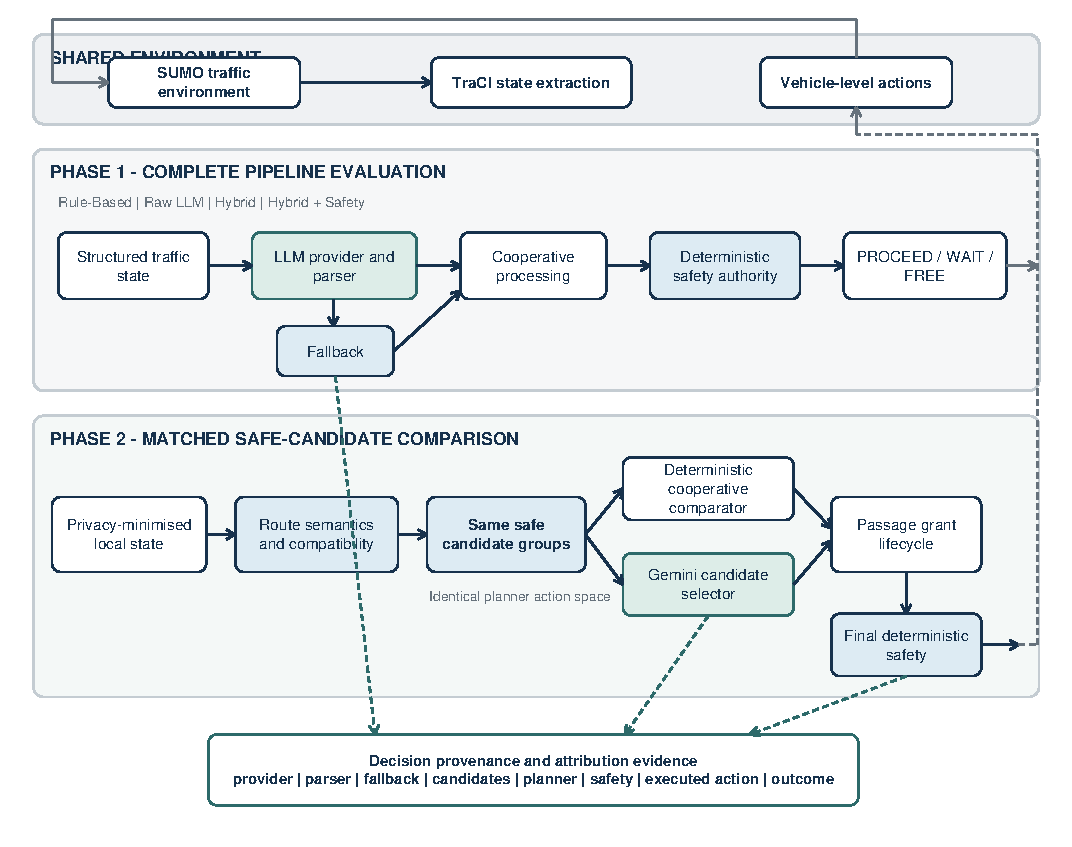
\includegraphics[width=0.98\textwidth]{figures/unified_architecture.pdf}

\caption{Unified attribution-aware architecture. Phase~1 evaluates complete action pipelines, whereas Phase~2 compares two selectors over identical deterministic safe candidate groups. Decision provenance records the path to executed actions and closed-loop outcomes.}

\label{fig:architecture}

\end{figure*}



\subsection{Traffic-State Representation}



Traffic state is extracted from TraCI once per simulation update. The common internal representation records vehicle identifier, local route identifier, immediate incoming and outgoing edges, intended movement, speed, distance to the intersection, estimated time to intersection, waiting time, and whether the vehicle lies inside the circular control zone. The control radius is 45~m. Time to intersection is an estimate derived from the current local motion state; non-finite estimates are represented as unavailable rather than supplied to the planner as artificial numerical values.



Phase~1 uses this state to build per-vehicle \texttt{PROCEED}, \texttt{WAIT}, or \texttt{FREE} decisions. Phase~2 derives a privacy-minimised planner view containing a temporary local vehicle identifier, immediate incoming and outgoing edge, \texttt{LEFT}/\texttt{STRAIGHT}/\texttt{RIGHT} movement, waiting time, speed, distance, finite time-to-intersection estimate where available, and control-zone status. Only vehicles represented in the current candidate set are included in the candidate-selection context.



The Gemini candidate selector is not given a vehicle origin, final destination, complete navigation route, route history, or unrelated repository and simulation information. Immediate incoming and outgoing edges are retained because they define the local intersection movement needed to interpret a candidate. This minimisation reduces unnecessary exposure while preserving the information required for local passage-group selection; it is an engineering restriction rather than a formal privacy guarantee.



Request-level and vehicle-level evidence remain distinct. One logical request can describe several vehicles and yield one group selection that is subsequently converted into multiple vehicle actions. Vehicles outside the control zone are handled by the deterministic interface. Request counts are therefore not inferred from the number of vehicle trace rows.



\subsection{Mixed-Turn Route Semantics and Conflict Model}



The SUMO network contains four incoming approaches, denoted \texttt{N}, \texttt{E}, \texttt{S}, and \texttt{W}, and the corresponding outgoing edges. Phase~2 derives movement semantics from the actual connection direction stored in \texttt{net.net.xml}. Each incoming approach supports a right turn, straight movement, and left turn, giving 12 local routes: \texttt{N\_W}, \texttt{N\_S}, \texttt{N\_E}, \texttt{E\_N}, \texttt{E\_W}, \texttt{E\_S}, \texttt{S\_E}, \texttt{S\_N}, \texttt{S\_W}, \texttt{W\_S}, \texttt{W\_E}, and \texttt{W\_N}. Resolving the immediate edge pair to \texttt{LEFT}, \texttt{STRAIGHT}, or \texttt{RIGHT} provides the deterministic basis for conflict reasoning and candidate generation.



Compatibility is defined over route movements rather than vehicle identifiers. Under the frozen model, repeated vehicles on the same route are compatible, right turns from distinct approaches are compatible, straight movements from opposite approaches are compatible, and left turns from opposite approaches are compatible. Other route combinations are treated as conflicting. The model is intentionally conservative: it can reject simultaneous movements that may be geometrically feasible under more detailed lane-level reasoning. Lane-level compatibility is outside the implemented method, so the abstraction favours transparent, reproducible conflict exclusion over maximal intersection throughput and does not enumerate every physically safe combination.



\subsection{Safe Candidate Passage Groups}



Candidate generation runs before either Phase~2 planner. It considers only vehicles inside the control zone with a resolvable supported route. Relevant states are ordered deterministically by time to intersection and vehicle identifier. The generator includes every relevant singleton, compatible vehicle pairs, and larger groups constructed from mutually compatible movements. Every emitted group is checked pairwise, so no candidate contains an internal conflict under the frozen route-level abstraction.



Candidate identifiers are stable concatenations of their vehicle identifiers. Candidate features include group size, aggregate waiting time, maximum individual waiting time, minimum time to intersection, and a movement summary. Candidate generation is a deterministic constraint on the planner's action space rather than a request for Gemini to calculate geometry. Both planners receive the same candidate set, and neither can authorize a group that the compatibility model did not admit.



Table~\ref{tab:controllers} locates the six evaluated controller and planner configurations within this shared architecture.

\begin{table}[t]

\centering

\caption{Evaluated decision configurations within the shared execution architecture.}

\label{tab:controllers}

\renewcommand{\arraystretch}{1.08}

\begin{tabular}{p{1.75cm} p{3.5cm}}

\toprule

\textbf{Controller} & \textbf{Enabled stages} \\

\midrule

Rule-Based & Deterministic interface rule only \\

Raw LLM & LLM proposal, parsing, validation, fallback \\

Hybrid & Raw LLM + cooperative post-processing \\

Hybrid + Safety & Hybrid + deterministic safety verification \\

Deterministic candidate & Safe candidates + cooperative comparator + grant + safety \\

Gemini candidate & Safe candidates + Gemini selection/comparator fallback + grant + safety \\

\bottomrule

\end{tabular}

\end{table}



\subsection{Prompt Construction and Structured LLM Interface}



Phase~1 converts the structured traffic state and deterministic policy hints into a frozen prompt defining the legal \texttt{PROCEED}, \texttt{WAIT}, and \texttt{FREE} actions and required machine-readable response. The model is asked for high-level vehicle decisions rather than trajectories or continuous control. Prompt wording and request configuration are treated as experimental configuration, because modifying them between runs would change the controller being evaluated.



Phase~2 uses a different but equally constrained contract. The frozen provider and model are Google Gemini and \texttt{gemini-3.6-flash} in fixed-provider research mode. Gemini receives the same privacy-minimised traffic snapshot and exact deterministic candidate groups used to compute the comparator selection. Its only requested decision is a JSON object of the form \texttt{\{"selected\_candidate\_id":"<candidate\_id>"\}}. The structured response schema restricts the value to candidate identifiers supplied in that request.



This contract makes candidate selection, rather than deterministic conflict calculation, the model's experimental role. Gemini cannot invent a vehicle identifier, authorize a group outside the candidate set, or directly emit arbitrary simulator actions. Provider credentials are resolved outside the prompt and are neither included in the planner state nor persisted in the dissertation evidence.



\subsection{Parsing, Validation, and the Raw LLM Path}



A successful provider request influences the simulation only if its content passes the corresponding parser. Phase~1 validation checks that the response can be mapped to the expected vehicle identifiers and legal action vocabulary. Raw LLM then applies the minimum deterministic interface needed for executable actions; it is the least augmented LLM-assisted configuration rather than unrestricted model control of SUMO.



Phase~2 validation requires one object containing exactly one supplied candidate identifier. Malformed JSON, a missing identifier, multiple identifiers, or an unknown identifier is invalid. Provider success and parser success are recorded separately because a network response can arrive without satisfying the executable contract. A valid Gemini identifier is converted deterministically into \texttt{PROCEED} for members of that group, \texttt{WAIT} for competing controlled vehicles, and \texttt{FREE} outside the control zone.



The live-provider interface records provider and model identity, request status, parser status, failure classification, and latency separately from traffic outcomes. This separation prevents episode completion or efficient fallback behaviour from being counted as successful LLM reasoning.



\subsection{Deterministic Fallback Policy}



Both phases retain deterministic recovery for provider failure, timeout, or invalid output. In Phase~1, fallback applies a priority-and-compatibility policy over the current traffic state and can produce meaningful \texttt{PROCEED}, \texttt{WAIT}, and \texttt{FREE} actions. It is not an all-\texttt{WAIT} emergency behaviour and is not the standalone Rule-Based baseline. The baseline is an independently evaluated controller; fallback is an internal mechanism within the model-facing pipeline.



In Phase~2, the deterministic cooperative comparator is also the fallback for failed or invalid Gemini candidate selection. It operates over the same candidate set supplied to Gemini, and the resulting candidate receives a normal passage grant. Fallback reason, final candidate, and selection source are preserved independently. This design maintains episode progress while making clear whether a grant came from Gemini or deterministic recovery.



Fallback is consequently both an operational safeguard and an attribution variable. Traffic outcomes from a fallback-capable pipeline are not credited to live-LLM reasoning unless provider, parser, and selection provenance establish that the model produced the executed choice.



Table~\ref{tab:phase1_semantic_overlap} compares the frozen Phase~1 prompt and fallback. The prompt did not reproduce the complete fallback algorithm, but exposed substantial deterministic structure.

\begin{table*}[t]

\centering

\caption{Semantic overlap between the frozen Phase~1 prompt interface and deterministic control stages.}

\label{tab:phase1_semantic_overlap}

\renewcommand{\arraystretch}{1.07}

\scriptsize

\begin{tabular}{p{1.9cm} p{3.5cm} p{3.6cm} p{3.2cm}}

\toprule

\textbf{Policy element} & \textbf{Prompt/model information} & \textbf{Deterministic fallback behaviour} & \textbf{Attribution implication} \\

\midrule

Control-zone gating & Requires vehicles outside the control zone to be \texttt{FREE}. & Assigns \texttt{FREE} outside the zone. & High overlap; this action is fixed deterministically. \\

Priority vehicle & Receives a policy hint identifying the minimum-time-to-intersection vehicle and route. & Computes the controlled vehicle with minimum time to intersection. & High overlap in priority information. \\

Waiting-time priority & Contains no explicit waiting-time priority rule. & Does not rank vehicles by waiting time; priority uses time to intersection. & Low overlap on waiting-based fairness. \\

Route conflict and compatibility & Receives the deterministic conflict matrix and routes compatible with the priority route. & Applies the same deterministic compatibility predicate to the priority route. & High overlap in feasibility structure. \\

Cooperation & May return multiple simultaneous actions but is not instructed with the full fallback loop. & Allows the priority vehicle and compatible controlled vehicles to \texttt{PROCEED}. & Partial overlap; implementation remains distinct. \\

Action semantics & Is restricted to \texttt{PROCEED}, \texttt{WAIT}, and \texttt{FREE}. & Emits the same three actions. & High overlap in the executable action space. \\

Safety constraints & Receives conflict information but not the complete verifier algorithm. & Uses route compatibility; final verification is a separate stage. & Partial overlap, not algorithmic identity. \\

Tie-breaking & Receives the already computed priority identifier; no explicit tie rule is requested. & Stable input order resolves equal minimum-time values. & Deterministic choice is exposed without teaching the tie mechanism. \\

Provider/parser failure & The prompt does not define recovery behaviour. & Failure or invalid output invokes fallback. & No semantic overlap; this is runtime recovery. \\

Cooperative postprocessor & Has no authority over the later Hybrid stage. & Can promote compatible \texttt{WAIT} actions to \texttt{PROCEED}. & A separate deterministic contribution. \\

Final safety authority & Does not execute or verify simulator actions. & Hybrid + Safety can downgrade unsafe simultaneous passage. & A separate deterministic authority. \\

\bottomrule

\end{tabular}

\end{table*}



This overlap plausibly contributed to behavioural similarity, but Phase~1 cannot establish it as the sole cause; fallback dominance and absent downstream intervention also weaken attribution. Phase~2 responds by giving Gemini and the comparator identical safe candidates and comparing their identifiers in independent matched episodes. Because candidate construction remains deterministic, it improves rather than eliminates attribution.



\subsection{Cooperative Processing and Deterministic Comparator}



The Phase~1 Hybrid controller applies deterministic cooperative post-processing after the model-facing decision or its fallback. It identifies the controlled vehicle with minimum time to intersection and can promote compatible waiting vehicles to \texttt{PROCEED}. Raw and postprocessed decisions are retained separately, allowing the additional deterministic stage to be evaluated rather than assumed effective from its presence.



Phase~2 replaces that incremental post-processing question with an explicit deterministic cooperative comparator over safe candidates. The comparator ranks candidates lexicographically by: (1) larger group size, (2) higher aggregate waiting time, (3) higher maximum individual waiting time, (4) lower minimum time to intersection, and (5) ascending stable candidate identifier. The first candidate in this deterministic ordering is selected.



The comparator is a strong, reproducible counterfactual planner because it uses all candidate features defined by the method and always produces the same ranking for the same state. It is not claimed to be globally optimal or to encode the uniquely correct traffic objective. Its group-size-first preference explicitly prioritises simultaneous progress and is therefore important when later interpreting cases in which Gemini selects a smaller legal group.



\subsection{Gemini Candidate Selection}



The Phase~2 Gemini candidate selector receives the identical local snapshot and safe-candidate features used to compute the comparator ranking. Google Gemini with the fixed \texttt{gemini-3.6-flash} model returns one supplied candidate identifier under the structured schema described above. A valid response selects that candidate even when it differs from the comparator; agreement and disagreement are recorded rather than resolved by silently replacing the model choice.



Provider failure, request timeout, malformed output, or an identifier outside the candidate set invokes the deterministic comparator fallback. The final candidate is then converted through the common action interface and safety stage. This preserves a controlled comparison: Gemini provides high-level choice among safe alternatives, while geometry, candidate legality, action conversion, and final safety remain deterministic.



\subsection{Grant Lifecycle and Decision Epochs}



A Phase~2 planner decision occurs only when no passage grant is active and at least one legal candidate exists. This event defines a \emph{decision epoch}. The chosen candidate becomes an active grant: selected vehicles retain \texttt{PROCEED}, competing vehicles inside the control zone retain \texttt{WAIT}, and vehicles outside the zone remain \texttt{FREE}. Gemini is therefore called once per new Gemini-controlled epoch rather than once per SUMO simulation step.



The grant persists until all granted vehicles have left the control zone or the simulation. Persistence prevents per-step planner oscillation and gives each selection an observable execution interval. A fixed timeout closes a grant after 45 simulation seconds. The timeout update deliberately applies \texttt{WAIT} to all controlled vehicles once, after which a new candidate set can trigger replanning on the next update.



During synchronous Gemini inference, the controller does not advance SUMO simulation time. Provider wall-clock latency therefore does not directly lengthen the simulated episode, although it remains relevant to practical real-time deployment. Safety verification continues on every update during the grant, independently of whether a new planner call occurs.



\subsection{Deterministic Safety Verification and Execution Authority}



The Phase~1 Hybrid + Safety controller places deterministic verification after cooperative processing. The verifier examines simultaneous \texttt{PROCEED} actions using route conflict and time-to-intersection conflict detection, retains the earliest relevant priority where necessary, and can downgrade another action to \texttt{WAIT}. Raw, postprocessed, and final decisions are recorded separately.



Phase~2 has two deterministic safety boundaries with different roles. Safe candidate generation constrains the available choices before planner selection. After the chosen candidate has been converted to vehicle actions, the existing safety verifier remains final execution authority and is reapplied on every controlled update, including while a grant is active. A safety downgrade does not erase the selected-candidate record or automatically terminate the grant; normal clearance or timeout still governs the grant lifecycle.



The method records intervention rather than assuming empirical effectiveness. Collision-free operation alone cannot establish that the verifier caused the outcome, and the Results must report whether the verifier actually changed any actions.



\subsection{Diagnostics and Decision Provenance}



Phase~1 provenance records provider attempts and outcomes, parser success, fallback, raw and validated actions, cooperative modification, safety intervention, final action, source, and request timing. This permits a completed episode to be separated from successful provider operation and prevents fallback-generated decisions from being counted as live-model reasoning.



Phase~2 adds one canonical record per decision epoch. Conceptually, the record contains the privacy-minimised input, candidate set and features, deterministic comparator choice, Gemini choice, redacted response evidence, provider and parser status, fallback and final selection, grant source and lifecycle, intended and final actions, safety intervention, latency, token usage, and prompt hash with reconstruction inputs. Credentials and excluded navigation information are not part of this record.



This evidence reconstructs each disagreement from common state through both planner selections to the actions executed during the grant. It also preserves the distinction between request-level reliability, candidate-level agreement, and vehicle-level action execution. Provenance establishes traceability; causal traffic comparison additionally requires independent closed-loop episodes in which each planner can change its own subsequent SUMO state.



\subsection{Reproducibility and Evidence Preservation}



Controller configuration, scenario and scale, seed, provider and model, request parameters, traffic metrics, decision traces, and run-validation status are preserved as experiment artefacts. Phase~1 evidence validation checks executed scenario content rather than accepting run labels alone; this process excluded the invalid nominal 8V evidence and retained the corrected matrix described in Section~\ref{sec:experimental_design}.



Phase~2 additionally stores a deterministic initial-demand signature over scenario, seed, routes, departure times, and car-following configuration. A paired comparison is accepted only when the comparator and Gemini episodes have matching signatures and valid independent run artefacts. Prompt hashes and reconstruction inputs preserve the model-facing decision context without persisting credentials.



The evidence hierarchy separates formal closed-loop traffic outcomes, offline decision analysis, integration smoke evidence, and software validation. This prevents supporting diagnostics from being retroactively counted as formal episodes or observer-trajectory metrics from being interpreted as planner-controlled traffic effects.



The preserved local experiment environment identifies SUMO 1.27.0. The Phase~2 formal workflow used the canonical Python 3.10.11 environment and the frozen Google Gemini \texttt{gemini-3.6-flash} configuration. The network is defined by \texttt{net.net.xml}; the targeted generator derives route and \texttt{simulation.sumocfg} files from the declared scenario, scale, and seed. Appendix Table~\ref{tab:repro_summary} consolidates the minimum reproduction contract without exposing credentials or machine-specific secret locations.



\section{Experimental Design}

\label{sec:experimental_design}



\subsection{Phase 1 Experimental Design}



\subsubsection{Experimental Matrix}



The formal experiment was designed to compare complete controller configurations under a common simulation environment while varying controller architecture and traffic scale. Four controllers were evaluated: Rule-Based, Raw LLM, Hybrid, and Hybrid + Safety. Each controller was tested in four-vehicle (4V) and eight-vehicle (8V) scenarios using three random seeds, producing a retained formal matrix of \(4\ \text{controllers} \times 2\ \text{scales} \times 3\ \text{seeds} = 24\ \text{runs}\).



The Rule-Based configuration provides the standalone deterministic baseline. Raw LLM represents the least augmented model-facing pipeline, including the deterministic mechanisms required for valid execution and recovery from provider failure. Hybrid adds cooperative post-processing, while Hybrid + Safety additionally applies deterministic safety verification. Keeping the simulation environment and high-level action interface consistent across these configurations allows differences to be examined at both the complete-pipeline level and, where diagnostic evidence permits, the internal component level.



The two traffic scales provide a limited test of how controller behaviour changes as the number of interacting vehicles increases. The 4V scenario provides the smaller coordination case, while 8V increases the number of vehicles competing for the intersection and therefore the opportunity for waiting and interaction. The experiment is not intended to establish general scalability across arbitrary traffic density. Instead, the 4V--8V comparison provides evidence about robustness within the tested low-density scenario range.



The Phase~1 matrix contributes to the final research questions without answering all of them independently. It directly supports the pipeline comparison and attribution boundary in RQ1. The Raw LLM--Hybrid and Hybrid--Hybrid + Safety comparisons provide precursor evidence for the cooperative and safety questions later refined in RQ2 and RQ3. The 4V--8V comparison provides the initial bounded scale evidence that is subsequently extended, but not converted into a general scalability claim, under RQ4.



\subsubsection{Scenario Control and Repeated Runs}



All controller configurations operate within the same SUMO-based intersection-control framework. The evaluated scenarios use the same intersection environment and controller action semantics so that the principal experimental differences arise from controller configuration, scale, and seed rather than from changes to the underlying simulation architecture.



Three seeds are retained for each controller--scale combination. Repeated seeds provide limited information about run-to-run variation and prevent the comparison from depending entirely on a single execution. However, three runs per cell are insufficient for strong population-level statistical inference. The results are therefore interpreted descriptively rather than as statistical proof of superiority.



This distinction is important because several reported differences are numerically large, particularly in operational waiting and mean speed. Percentage changes and differences may be reported to describe the magnitude of the observed effect, but they are not treated as hypothesis-test results. Claims are consequently restricted to the retained scenarios and seeds.



\subsubsection{Phase 1 Metrics}



The evaluation combines traffic-level metrics with pipeline-level diagnostics. Traffic metrics measure the behaviour of the complete controller in the simulation, whereas pipeline diagnostics describe how the LLM-assisted architecture produced those outcomes.



The primary traffic metrics are completion rate, operational waiting, mean speed, throughput, and collision count. Completion rate measures the proportion of expected vehicles that successfully complete the scenario, while throughput describes completed traffic relative to the simulated episode. Mean speed provides a measure of overall vehicle progress.



Operational waiting is used as the principal delay-related metric. In this implementation it is derived from stop-like occupancy in the recorded simulation trace and should therefore be interpreted as an operational proxy for waiting rather than as a general queueing-delay measure. This definition is retained consistently across controller comparisons.



Collision count provides a basic safety outcome but is interpreted conservatively. If all controllers complete the tested scenarios without collision, the metric becomes saturated and cannot by itself distinguish the effectiveness of different safety mechanisms. Internal safety interventions must therefore also be considered when assessing the Hybrid + Safety configuration.



For LLM-assisted controllers, provider-level metrics include logical request count, provider-request success, parser success, fallback activation, and request latency. Cooperative intervention and safety-override records are additionally retained for the corresponding controller stages. These metrics allow strong traffic performance to be distinguished from reliable live-model operation.



Traffic and provider metrics are not assumed to share the same denominator. A logical provider request may generate decisions for multiple vehicles, while vehicle-level trace rows describe individual executed or interface-level actions. Provider reliability is therefore evaluated at the logical-request level wherever request provenance is available, whereas decision agreement and action attribution are evaluated using aligned vehicle-level records.



\subsubsection{Formal Evidence Validation}



The final formal dataset was established through validation of the executed scenario evidence rather than relying solely on experiment directory names. The initial formal experiment set, denoted internally as \texttt{formal\_v2}, contained valid 4V runs. During subsequent evidence auditing, however, the runs nominally labelled as 8V were found not to provide valid eight-vehicle evidence: the underlying scenario and trace information indicated that the intended scale had not been executed correctly.



Those nominal 8V results were therefore excluded from the retained evidence rather than being analysed as genuine eight-vehicle experiments. Corrected 8V runs were subsequently generated under the intended configuration and retained as \texttt{formal\_v4}. The final 24-run formal matrix consequently combines the validated 4V evidence from \texttt{formal\_v2} with the corrected 8V evidence from \texttt{formal\_v4}.



This replacement is treated as an experimental-validity correction rather than a performance-based selection. The invalid runs were rejected because their executed scenario did not match the experimental condition represented by their labels, not because their outcomes were favourable or unfavourable. The retained evidence boundary is fixed before the final comparison and is applied consistently to all four controller configurations.



\subsubsection{Formal and Post-hoc Evidence Boundary}



The 24 retained runs constitute the Phase~1 formal experiment used for the primary controller comparison. The later Phase~1 Gemini diagnostic and fallback-only analyses are not added to this matrix. They were conducted after the formal results exposed an attribution problem: traffic performance remained strong in the LLM-assisted pipelines despite very low live-provider success.



Those post-hoc experiments therefore answer a narrower diagnostic question. Their purpose is to test whether removing provider failure reveals behaviour that differs from deterministic fallback, rather than to increase the Phase~1 formal sample size or replace the original controller comparison. Phase~1 formal traffic results and post-hoc attribution evidence are consequently reported separately from each other and from the Phase~2 formal closed-loop matrix.



This separation preserves the interpretation of the study. The formal experiment evaluates the performance and reliability of the complete controller configurations under the retained experimental conditions. The supplementary analysis investigates why those results occurred and how much evidence they provide for an independent LLM contribution.



\subsection{Phase 2 Experimental Design}



Phase~2 retains the established SUMO execution, action interface, fallback availability, safety authority, and provenance architecture. Its experimental change is to compare the Gemini candidate selector with the deterministic cooperative comparator over identical safe candidates in situations designed to expose more than one legal high-level choice.



\subsubsection{Two-Layer Evaluation Design}



The first layer is \emph{offline paired decision analysis}. Both planners inspect the same recorded privacy-minimised state and candidate set. This supports analysis of candidate preference, agreement or disagreement, provider and parser operation, fallback, counterfactual safety handling, latency, and token usage. The observed traffic trajectory belongs to the controller that generated the recorded state; offline comparison does not make the unexecuted planner responsible for completion, waiting, speed, or episode duration.



The second layer is \emph{independent closed-loop paired controller evaluation}. For each scenario and seed, one SUMO episode is controlled by the deterministic comparator and a separate SUMO episode is controlled by the Gemini candidate selector. Initial demand is matched, but each planner applies its own grants and can therefore change subsequent vehicle states, candidate sets, and episode outcomes. Only this layer supports causal comparison of planner-controlled traffic within the evaluated pair.



\subsubsection{Targeted Mixed-Turn Scenarios}



Four targeted scenario classes create distinct local decision contexts. Their routes and departure structure are specified explicitly rather than sampled from a generic demand distribution. Table~\ref{tab:phase2_scenarios} summarises their methodological roles and formal scales.

\begin{table*}[t]

\centering

\caption{Phase~2 targeted scenarios and formal scale conditions.}

\label{tab:phase2_scenarios}

\renewcommand{\arraystretch}{1.08}

\begin{tabular}{p{1.1cm} p{4.3cm} p{8.0cm}}

\toprule

\textbf{Class} & \textbf{Formal scale} & \textbf{Methodological purpose} \\

\midrule

S1 & 8V & Balanced mixed-turn reference with distributed arrivals and all three movement classes. \\

S2 & 8V & Clustered near-simultaneous arrivals that create competing conflicting movements. \\

S3 & 8V and 12V & Cooperative opportunity with multiple compatible movements and competing larger safe groups. \\

S4 & 8V and 16V & Fairness pressure in which a waiting left-turn movement competes with alternative legal groups. \\

\bottomrule

\end{tabular}

\end{table*}



The scenario labels describe design intent rather than experimental outcome. In particular, S4 creates waiting pressure but does not assume that either planner improves fairness, and S2 creates clustered departures without assuming that every observed state has a finite or identical time-to-intersection estimate.



\subsubsection{Formal Closed-Loop Matrix}



The formal conditions are S1 8V, S2 8V, S3 8V, S4 8V, S3 12V, and S4 16V. Each condition is evaluated with seeds 1, 2, and 3 under both planners. The complete design is therefore

\[
6\ \text{conditions} \times 3\ \text{seeds} \times 2\ \text{planners}
= 36\ \text{independent closed-loop episodes}.
\]

This gives 18 matched scenario--seed pairs and 18 episodes per planner. The matrix is a targeted small-sample comparison rather than a large-sample traffic study. Native static signal control is neutralised during candidate-controlled episodes so that the reported behaviour is produced by the candidate planner, grant execution, and retained deterministic safety layer rather than an unreported third controller.



\subsubsection{Seed and Paired-Condition Semantics}



Targeted route assignment is fixed within each scenario. In S1 and S3, the seed controls a bounded zero-to-one-second departure jitter and SUMO's stochastic car-following behaviour with \(\sigma=0.5\). In S2 and S4, routes and departure offsets remain exact; seed variation comes from SUMO car-following behaviour rather than redrawn traffic demand. The three seeds are therefore trajectory replicates under the declared scenario semantics, not three fully independent samples from an unrestricted demand population.



For each paired condition, planners use the same scenario class, vehicle count, route and departure specification, seed semantics, network, vehicle parameters, and initial-demand signature. The episodes run in independent SUMO processes. Planner-specific grants can then produce different subsequent trajectories without contaminating the matched initial condition. This supports within-pair causal interpretation while leaving external generalisation bounded by the handcrafted scenarios and small seed count.



\subsubsection{Phase 2 Metrics and Statistical Boundary}



Traffic metrics are completion, throughput, mean waiting time, maximum waiting time, mean speed, episode duration, and collision count. Planner and control metrics are decision epochs, grants, grant duration, grant timeouts, and safety interventions. Gemini reliability metrics are provider success, parser success, fallback, request latency, and prompt, completion, and total token usage. Attribution metrics are comparator selection, Gemini selection, agreement or disagreement, final selected candidate, and selection source.



Gemini inference is synchronous: SUMO simulation time does not advance while the request is pending. Request latency therefore measures experiment wall-clock and deployment cost rather than simulated traffic delay. It is reported separately from episode duration.



Three seeds per condition support descriptive paired evidence. Means, sample standard deviations, ranges, and Gemini-minus-comparator paired deltas can summarise the observed runs. The design does not support strong inferential statistical claims, unrestricted scale claims, or broad generalisation, and no hypothesis test is introduced solely from this sample size.



\section{Results}



\subsection{Phase 1 Results}



\subsubsection{Formal Traffic Performance and Bounded Scale Comparison}



Table~\ref{tab:formal_traffic} summarises the retained 24-run Phase~1 traffic boundary: four controllers, 4V and corrected 8V conditions, and three seeds per controller--scale combination. All configurations completed every planned vehicle and recorded zero collisions. Throughput therefore equalled the requested vehicle count in each retained run.



In 4V, Rule-Based operational waiting was 82.0 steps and mean speed was 2.31~m/s, compared with 15.0 steps and 6.80~m/s for each LLM-assisted pipeline. In corrected 8V, Rule-Based mean waiting increased to 242.04 steps and mean speed decreased to 1.19~m/s, while the three LLM-assisted pipelines recorded approximately 15.29 steps and 6.60~m/s. Raw LLM, Hybrid, and Hybrid + Safety were indistinguishable on these aggregate traffic measures.



These observations establish a descriptive advantage for the complete fallback-capable LLM-assisted pipelines over the selected Rule-Based baseline in the evaluated traffic conditions. They do not identify the live model as the cause of that difference. The 4V--8V change is also a bounded comparison within one intersection and does not establish general scalability.






\begin{table*}[t]

\centering

\caption{Formal traffic performance in the retained evidence boundary. Waiting and speed are mean $\pm$ sample standard deviation across the three retained seeds; completion and collisions are the common per-run outcomes.}

\label{tab:formal_traffic}

\renewcommand{\arraystretch}{1.1}

\begin{tabular}{p{2.75cm} p{0.9cm} p{2.25cm} p{2.05cm} p{1.35cm} p{1.15cm}}

\toprule

\textbf{Controller} & \textbf{Scale} & \textbf{Operational waiting} & \textbf{Mean speed} & \textbf{Completion} & \textbf{Collisions} \\

\midrule

Rule-Based & 4V & 82.0 $\pm$ 0.0 & 2.3098 $\pm$ 0.0000 m/s & 100\% & 0 \\

Rule-Based & 8V & 242.0417 $\pm$ 135.4396 & 1.1895 $\pm$ 0.9230 m/s & 100\% & 0 \\

Raw LLM & 4V & 15.0 $\pm$ 0.0 & 6.8026 $\pm$ 0.0000 m/s & 100\% & 0 \\

Raw LLM & 8V & 15.2917 $\pm$ 2.5042 & 6.5991 $\pm$ 0.3111 m/s & 100\% & 0 \\

Hybrid & 4V & 15.0 $\pm$ 0.0 & 6.8026 $\pm$ 0.0000 m/s & 100\% & 0 \\

Hybrid & 8V & 15.2917 $\pm$ 2.5042 & 6.5991 $\pm$ 0.3111 m/s & 100\% & 0 \\

Hybrid + Safety & 4V & 15.0 $\pm$ 0.0 & 6.8026 $\pm$ 0.0000 m/s & 100\% & 0 \\

Hybrid + Safety & 8V & 15.2917 $\pm$ 2.5042 & 6.5991 $\pm$ 0.3111 m/s & 100\% & 0 \\

\bottomrule

\end{tabular}

\end{table*}



Episode duration showed the same pattern. Rule-Based recorded 114.000 $\pm$ 0.000~s at 4V and 344.000 $\pm$ 150.9006~s at 8V. Each LLM-assisted pipeline recorded 52.000 $\pm$ 0.000~s at 4V and 105.333 $\pm$ 0.577~s at 8V, using sample standard deviations across seeds.



\subsubsection{Provider Reliability and Fallback Dependence}



Table~\ref{tab:provider_reliability} reports provider reliability for the retained Phase~1 traffic boundary. Counts are logical provider requests, not replicated vehicle-level trace rows; one provider response may appear in multiple vehicle records.

\begin{table*}[t]
\centering
\caption{Logical-request provider reliability in the retained Phase~1 formal traffic boundary. Parser success is conditional on provider success.}
\label{tab:provider_reliability}
\scriptsize
\renewcommand{\arraystretch}{1.08}
\begin{tabular}{p{2.2cm} p{0.7cm} p{1.6cm} p{1.6cm} p{1.45cm} p{1.25cm} p{2.25cm}}
\toprule
Controller & Scale & Logical requests & Provider success & Parser success & Fallback & Success / fallback rate \\
\midrule
Raw LLM & 4V & 159 & 10 & 10/10 & 149 & 6.29\% / 93.71\% \\
Raw LLM & 8V & 319 & 2 & 2/2 & 317 & 0.63\% / 99.37\% \\
Hybrid & 4V & 159 & 9 & 9/9 & 150 & 5.66\% / 94.34\% \\
Hybrid & 8V & 319 & 1 & 1/1 & 318 & 0.31\% / 99.69\% \\
Hybrid + Safety & 4V & 159 & 9 & 9/9 & 150 & 5.66\% / 94.34\% \\
Hybrid + Safety & 8V & 319 & 1 & 1/1 & 318 & 0.31\% / 99.69\% \\
\bottomrule
\end{tabular}
\end{table*}

Separately, the broader Phase~1 provider sweep contained 2,664 replicated vehicle-level trace rows marked as provider attempts, including nominal 8V traces excluded from retained eight-vehicle traffic evidence. Of those rows, 109 recorded provider and parser success and 2,555 recorded fallback. These row-level diagnostics are not the denominator used in Table~\ref{tab:provider_reliability}.






Both populations show fallback dominance, explaining how traffic completion could remain high despite poor provider operation. This also fixes the attribution boundary: the Phase~1 traffic advantage characterises the complete fallback-capable architecture and cannot be assigned independently to successful live-model reasoning.



Log-level comparison confirmed that Raw LLM, Hybrid, and Hybrid + Safety produced identical effective vehicle-action traces in every retained Phase~1 scale--seed condition, rather than merely equal rounded aggregates. For each controller, the 1,372 vehicle-step records contained identical totals of 473 \texttt{FREE}, 736 \texttt{PROCEED}, and 163 \texttt{WAIT} actions. Provider and fallback provenance differed in some records, but zero cooperative post-processing interventions and zero safety overrides meant that those upstream differences did not change executed actions. Fallback dominance, deterministic policy hints, and absent downstream intervention jointly limit attribution; the evidence does not isolate semantic overlap as the sole cause. Zero recorded collisions likewise cannot identify a safety-verifier effect.



\subsubsection{Post-hoc Gemini Attribution Analysis}



A post-hoc Raw LLM 4V seed-1 diagnostic tested whether reliable inference produced behaviour distinct from Phase~1 fallback. All 53 provider requests and parsers succeeded, no fallback occurred, all four vehicles completed, and no collision was recorded. This diagnostic remains outside the 24-run formal traffic matrix and is summarised in Table~\ref{tab:posthoc_attribution}.





\begin{table}[t]

\centering

\caption{Post-hoc attribution evidence for the reliable Gemini 4V seed1 diagnostic.}

\label{tab:posthoc_attribution}

\renewcommand{\arraystretch}{1.08}

\scriptsize

\begin{tabular}{p{1.4cm} p{1.3cm} p{0.9cm} p{1.0cm} p{1.5cm}}

\toprule

\textbf{Condition} & \textbf{Provider path} & \textbf{Waiting} & \textbf{Mean speed} & \textbf{Decision agreement} \\

\midrule

Reliable Gemini 4V seed1 & 53/53 success, 0 fallback & 11.0 & 7.58 m/s & 132/132 raw and final \\

Fallback-only 4V seed1 & deterministic fallback only & 11.0 & 7.58 m/s & matched action stream \\

High-discrimination subset & same diagnostic slice & -- & -- & 39/39 raw and final \\

\bottomrule

\end{tabular}

\end{table}





Reliable Gemini and fallback-only control both recorded 11.0 waiting steps and 7.58~m/s mean speed. Gemini matched fallback on all 132 aligned raw and final vehicle decisions, including all 39 decisions in the higher-discrimination subset. Reliable inference was therefore achieved without behavioural discrimination in the original state distribution. Phase~2 addresses that remaining attribution limitation through matched candidate-level and closed-loop comparison.



\subsection{Phase 2 Results}



Phase~1 produced strong pipeline outcomes but identical assisted-pipeline traces under fallback-dominated operation and substantial prompt--fallback overlap. Phase~2 directly compares candidate identifiers under reliable Gemini operation. Across seeds 1--3 and bounded 8V, 12V, and 16V conditions, 36 independent episodes and 93 Gemini epochs yielded 89 agreements and four differences. This exposes attributable planner divergence without claiming broad generalisation; all paired demand signatures matched, with no invalidation or retry.



\subsubsection{Paired Closed-Loop Traffic Outcomes}



Table~\ref{tab:phase2_traffic} reports means and sample standard deviations over three seeds. Waiting and duration are seconds, speed is metres per second, and each delta is the Gemini mean minus the deterministic-comparator mean. Deltas were calculated from the unrounded run values. Every episode completed its requested vehicle count, throughput equalled that count, and zero collisions were recorded. There were also zero safety interventions and zero grant timeouts.

\begin{table*}[t]

\centering

\caption{Phase~2 paired closed-loop traffic outcomes. Values are deterministic/Gemini mean $\pm$ sample standard deviation; $\Delta$ is Gemini minus deterministic.}

\label{tab:phase2_traffic}

\renewcommand{\arraystretch}{1.08}

\scriptsize

\begin{tabular}{p{1.15cm} p{2.65cm} p{0.72cm} p{2.65cm} p{0.72cm} p{2.65cm} p{0.72cm}}

\toprule

\textbf{Condition} & \textbf{Mean waiting D/G} & \textbf{$\Delta$} & \textbf{Mean speed D/G} & \textbf{$\Delta$} & \textbf{Duration D/G} & \textbf{$\Delta$} \\

\midrule

S1 8V & 9.75 $\pm$ 0.99 / 9.75 $\pm$ 0.99 & 0.00 & 7.31 $\pm$ 0.25 / 7.31 $\pm$ 0.25 & 0.00 & 73.33 $\pm$ 2.08 / 73.33 $\pm$ 2.08 & 0.00 \\

S2 8V & 11.17 $\pm$ 0.07 / 10.83 $\pm$ 0.62 & -0.33 & 7.16 $\pm$ 0.10 / 7.30 $\pm$ 0.30 & +0.14 & 54.67 $\pm$ 2.08 / 54.33 $\pm$ 2.52 & -0.33 \\

S3 8V & 6.71 $\pm$ 0.75 / 6.71 $\pm$ 0.75 & 0.00 & 7.79 $\pm$ 0.34 / 7.79 $\pm$ 0.34 & 0.00 & 45.67 $\pm$ 3.06 / 45.67 $\pm$ 3.06 & 0.00 \\

S4 8V & 5.79 $\pm$ 0.44 / 5.79 $\pm$ 0.44 & 0.00 & 8.21 $\pm$ 0.29 / 8.21 $\pm$ 0.29 & 0.00 & 44.00 $\pm$ 1.73 / 44.00 $\pm$ 1.73 & 0.00 \\

S3 12V & 8.14 $\pm$ 1.33 / 9.81 $\pm$ 1.10 & +1.67 & 7.31 $\pm$ 0.42 / 6.90 $\pm$ 0.31 & -0.41 & 54.00 $\pm$ 3.46 / 55.00 $\pm$ 3.00 & +1.00 \\

S4 16V & 9.60 $\pm$ 1.01 / 9.60 $\pm$ 1.01 & 0.00 & 7.25 $\pm$ 0.29 / 7.25 $\pm$ 0.29 & 0.00 & 66.33 $\pm$ 1.53 / 66.33 $\pm$ 1.53 & 0.00 \\

\bottomrule

\end{tabular}

\end{table*}



Four conditions produced identical means under both planners. S2 8V produced a small favourable descriptive Gemini difference: mean waiting was 0.33~s lower, mean speed was 0.14~m/s higher, and duration was 0.33~s shorter. S3 12V produced the opposite descriptive direction: Gemini mean waiting was 1.67~s higher, mean speed was 0.41~m/s lower, and duration was 1.00~s longer. These values are paired descriptive observations rather than inferential results.



\subsubsection{Gemini Reliability and Candidate Agreement}



Gemini made 93 formal requests. Provider success was 93/93, parser success was 93/93, and no deterministic fallback occurred. Gemini selected the same candidate as the deterministic comparator in 89 of 93 comparable formal decisions and a different legal candidate in four, giving 95.70\% agreement. Table~\ref{tab:phase2_reliability} shows that the disagreements were concentrated in S2 8V and S3 12V rather than distributed across all conditions.

\begin{table*}[t]

\centering

\caption{Phase~2 Gemini reliability, candidate agreement, token use, and mean provider latency by condition.}

\label{tab:phase2_reliability}

\renewcommand{\arraystretch}{1.08}

\footnotesize

\begin{tabular}{p{1.45cm} p{1.15cm} p{2.05cm} p{1.65cm} p{1.1cm} p{1.8cm} p{1.75cm}}

\toprule

\textbf{Condition} & \textbf{Requests} & \textbf{Provider/parser success} & \textbf{Agree/disagree} & \textbf{Fallback} & \textbf{Total tokens} & \textbf{Mean latency (ms)} \\

\midrule

S1 8V & 21 & 21/21; 21/21 & 21/0 & 0 & 19,673 & 10,766.15 \\

S2 8V & 15 & 15/15; 15/15 & 14/1 & 0 & 23,801 & 6,629.07 \\

S3 8V & 12 & 12/12; 12/12 & 12/0 & 0 & 21,633 & 4,986.85 \\

S4 8V & 12 & 12/12; 12/12 & 12/0 & 0 & 23,766 & 3,324.06 \\

S3 12V & 15 & 15/15; 15/15 & 12/3 & 0 & 50,363 & 8,359.63 \\

S4 16V & 18 & 18/18; 18/18 & 18/0 & 0 & 70,756 & 9,412.34 \\

\midrule

Total & 93 & 93/93; 93/93 & 89/4 & 0 & 209,992 & 7,742.72 \\

\bottomrule

\end{tabular}

\end{table*}



\subsubsection{Formal Disagreement Cases}



All four disagreements are accounted for in Table~\ref{tab:phase2_disagreements}. Each Gemini selection was a valid supplied candidate. None involved provider failure, parser failure, fallback, or safety intervention, and every selected grant cleared normally.

\begin{table*}[t]

\centering

\caption{All formal Gemini--comparator candidate disagreements.}

\label{tab:phase2_disagreements}

\renewcommand{\arraystretch}{1.08}

\footnotesize

\begin{tabular}{p{2.3cm} p{2.55cm} p{1.45cm} p{2.2cm} p{2.0cm}}

\toprule

\textbf{Condition, seed, time} & \textbf{Comparator/Gemini group} & \textbf{Legal candidates} & \textbf{Aggregate/max wait (s)} & \textbf{Gemini grant clearance} \\

\midrule

S2 8V, seed 1, $t=11$ & 2 vehicles / 2 vehicles & 10 & 6 / 2 & Cleared in 7~s \\

S3 12V, seed 1, $t=21$ & 4 vehicles / 2 opposite-straight & 18 & 38 / 10 & Cleared in 9~s \\

S3 12V, seed 2, $t=23$ & 4 vehicles / 2 opposite-straight & 18 & 56 / 13 & Cleared in 9~s \\

S3 12V, seed 3, $t=20$ & 4 vehicles / 2 opposite-straight & 18 & 30 / 10 & Cleared in 9~s \\

\bottomrule

\end{tabular}

\end{table*}



The S2 8V difference occurred once, in seed~1, and both planners selected legal two-vehicle groups. At condition level this coincided with the small favourable descriptive Gemini deltas reported above; it is not treated as a general S2 advantage.



In all three S3 12V seeds, the deterministic comparator selected a legal compatible four-vehicle group while Gemini selected a legal two-vehicle opposite-straight group. This was a genuine candidate preference rather than fallback, parsing, or safety modification. The repeated choice pattern coincided with the S3 12V descriptive deltas of +1.67~s mean waiting, -0.41~m/s mean speed, and +1.00~s episode duration for Gemini relative to the comparator.



No disagreement occurred in S3 8V, whereas one occurred in every evaluated S3 12V seed. In S4, Gemini matched the comparator in all 12 decisions at 8V and all 18 decisions at 16V, so no planner divergence was observed in either fairness-pressure condition. These are bounded condition observations: vehicle count, scenario composition, candidate structure, and timing are not independently varied.



\subsubsection{Latency, Tokens, and Evidence Boundary}



Across the 93 Gemini requests, provider latency had a mean of 7,742.72~ms, median of 3,819.84~ms, minimum of 1,050.98~ms, and maximum of 20,019.86~ms. These are wall-clock provider measurements. SUMO simulation advancement was paused during synchronous inference, so request latency did not directly increase simulated episode duration.



The requests used 205,347 prompt tokens and 4,645 completion tokens, for 209,992 tokens in total. No financial cost is inferred because the experiment did not freeze an authoritative pricing calculation.



The main Phase~2 results are the independent closed-loop outcomes, formal reliability evidence, decision agreement and disagreement, and reconstructed disagreement cases reported above. Offline observer analysis, the closed-loop smoke pair, intermediate Batch~1 reporting, complete per-seed records, raw decision JSON, and software-test inventories remain supporting evidence rather than additional formal traffic results.



\section{Discussion and Limitations}



\subsection{Integrated Interpretation of the Two Phases}



The two experimental phases answer different but connected questions. Phase~1 evaluated complete controller pipelines. Raw LLM, Hybrid, and Hybrid + Safety produced lower operational waiting and higher mean speed than the selected Rule-Based baseline in the retained 4V and corrected 8V conditions, with full completion and zero recorded collisions. This is a meaningful system-level result: the fallback-capable model-facing architectures were more effective than that baseline within the evaluated traffic conditions.



The provider evidence prevents this traffic advantage from being assigned independently to live-model reasoning. In the broader replicated-row provider sweep, 2,664 vehicle-level trace rows were marked as provider attempts and 2,555 as fallback, so deterministic recovery supplied most model-facing pipeline behaviour. A fallback-heavy architecture can therefore perform well and remain operational while providing weak evidence about the value added by the live model. Phase~1 did not fail; it exposed the distinction between pipeline performance and model contribution and thereby identified the attribution problem that the second phase was designed to resolve.



Phase~2 retained the same broad simulator, execution, provenance, fallback, and downstream safety architecture but changed the decision experiment. Reliable Gemini inference and a strong lexicographic deterministic comparator received the same privacy-minimised state and the same deterministically safe candidate groups. Their choices then controlled independent SUMO episodes from matched initial demand. This design made a model-specific contribution identifiable whenever the planners selected different candidates, while keeping feasibility calculations and final execution authority deterministic.



Operational reliability was materially different in the frozen Phase~2 matrix: all 93 provider requests and all 93 parser operations succeeded, and no fallback occurred. The formal Gemini choices are therefore attributable to the live model rather than deterministic substitution. This establishes operational reliability during the frozen matrix, not universal reliability across providers, models, prompts, or deployment conditions.



\subsection{Agreement, Divergence, and Closed-Loop Consequences}



Gemini selected the same candidate as the deterministic comparator in 89 of 93 comparable decisions, or 95.70\%. This substantial overlap is bounded by the frozen scenarios, prompt, compatibility model, and comparator. It shows that reliable model operation did not automatically create qualitatively different planning behaviour. It does not establish planner equivalence, imitation, or the general dispensability of LLM reasoning. The comparison is informative precisely because the comparator is not artificially weak: its lexicographic ranking explicitly favours larger legal groups before applying waiting, arrival, and stable tie-breaking criteria.



The four disagreements demonstrate behavioural identifiability. The S2 8V seed-1 disagreement involved two different legal two-vehicle candidates and coincided with small favourable descriptive Gemini deltas of 0.33~s lower mean waiting, 0.14~m/s higher mean speed, and 0.33~s shorter duration. One event across three seeds is insufficient to establish a general Gemini benefit, but it confirms that a legal model preference can propagate into a distinct closed-loop trajectory.



The S3 12V result provides stronger repeated evidence within one targeted condition. In every evaluated seed, the comparator selected a legal compatible four-vehicle group while Gemini selected a legal two-vehicle opposite-straight group. None of these decisions resulted from provider or parser failure, fallback, or safety override, and every grant cleared. The repeated choice pattern was associated with Gemini-minus-deterministic descriptive differences of +1.67~s mean waiting, -0.41~m/s mean speed, and +1.00~s episode duration. The result supports the bounded conclusion that the smaller Gemini selections were less efficient in this condition; it does not establish a general ordering between planners.



Methodologically, S3 12V matters because the planner difference was not confined to an unexecuted response. Multiple legal cooperative groups existed, the selected group became a grant, vehicles executed that grant, and the resulting state influenced later decisions and traffic outcomes. Independent matched episodes preserved the chain from selection through execution to closed-loop consequence. This is stronger attribution evidence than offline output disagreement, while remaining limited to the tested scenario and three seeds.



The intended fairness pressure in S4 did not create a planner distinction. Gemini and the comparator agreed at every formal decision in both S4 8V and S4 16V. The experiment therefore observed no distinct Gemini fairness behaviour, benefit, or harm in those conditions. A scenario designed to expose a trade-off does not guarantee that two planners will resolve it differently, and agreement here is not evidence of fairness equivalence.



The bounded scale observations are similarly conditional. S3 had no disagreement at 8V and repeated disagreement at 12V, whereas S4 had no disagreement at either 8V or 16V. More complex candidate configurations can expose planner differences, but vehicle count is not isolated from scenario composition, candidate structure, and timing. The evidence therefore supports neither a general claim that Gemini deteriorates with scale nor that deterministic planning scales better.



\subsection{Safety, Latency, and the Role of the LLM}



The architecture separates prevention from observation. Deterministic route compatibility restricts the LLM to supplied legal candidate groups, and deterministic verification retains final authority over vehicle actions. Zero collisions, zero safety interventions, and zero grant timeouts were recorded in the Phase~2 formal matrix. These results show that the evaluated episodes were collision-free and that all selected grants completed without invoking the final verifier. They do not show that the verifier prevented collisions or quantify an independent verifier benefit. One plausible architectural explanation is that conservative candidate generation removed many unsafe combinations before final verification could become necessary, but intervention-rich tests would be required to measure the downstream layer itself.



Provider latency remains a practical limitation despite perfect request completion in Phase~2. Mean latency was 7.74272~s, median latency was 3.81984~s, and the observed range was 1.05098--20.01986~s. SUMO advancement paused during synchronous requests, so this wall-clock delay did not inflate simulated episode duration. Real traffic cannot be paused. Synchronous multi-second inference is therefore incompatible with a claim of real-time readiness and would require a latency-tolerant or asynchronous design before practical deployment could be considered.



The experiments do not establish that an LLM is necessary for this bounded candidate-selection task. The strong deterministic comparator reproduced most choices without remote-provider delay, and the observed Gemini divergences did not demonstrate a general control or fairness advantage. The evidence instead supports a narrower role: an LLM can be inserted as a high-level selector inside a deterministic feasibility and safety envelope, with its actual contribution exposed through provenance and matched closed-loop comparison. Such use is most defensible where future tasks require contextual judgement not already captured by explicit heuristics, rather than as a replacement for deterministic mechanisms that already represent the decision well.



The principal contribution is consequently attribution-aware evaluation. The framework separates provider reliability, parsing, fallback, candidate feasibility, planner choice, safety intervention, and closed-loop consequence. This matters for LLM-assisted robotics because strong performance by a hybrid system does not by itself demonstrate useful model reasoning. Model-specific claims require evidence that the model operated, selected an identifiable action, retained that action through deterministic stages, and changed the executed trajectory or outcome.



\subsection{Final Answers to the Research Questions}



\subsubsection{Answer to RQ1}



Within the retained Phase~1 4V and corrected 8V conditions, the complete Raw LLM, Hybrid, and Hybrid + Safety pipelines achieved lower operational waiting and higher mean speed than the selected Rule-Based controller while all configurations completed. Because fallback dominated the model-facing paths, this is a pipeline-level advantage and does not establish an independent live-LLM contribution.



\subsubsection{Answer to RQ2}



Under reliable Phase~2 operation, Gemini agreed with the strong deterministic comparator on 89 of 93 candidate decisions and produced four identifiable legal differences. The single S2 difference coincided with a small favourable descriptive outcome, while the repeated S3 12V differences coincided with less efficient descriptive outcomes; the evidence demonstrates model-specific closed-loop contribution in those cases but no general Gemini advantage.



\subsubsection{Answer to RQ3}



Deterministic compatibility, validation, grant execution, and final safety verification constrained the action space and retained final execution authority in both phases. The Phase~2 matrix recorded zero collisions, safety interventions, and grant timeouts, so collision-free operation was observed but an independent empirical benefit from final safety-verifier intervention was not demonstrated.



\subsubsection{Answer to RQ4}



Most evaluated Phase~2 conditions produced identical planner decisions and outcomes, while S3 12V exposed repeated divergence not observed in S3 8V; S4 produced no divergence at either 8V or 16V. These are bounded scenario-and-scale observations, and no general law of scalability or vehicle-count effect can be inferred because scale and candidate structure were not independently varied.



\subsection{Relation to Existing Literature}



The Phase~1 pipeline result remains consistent with the motivation for cooperative management of a shared conflict region \cite{Dresner2008,Safarov2022,Zhao2025}. The more distinctive contribution, however, concerns how a hybrid controller should be evaluated. Work on language-model planning, embodied reasoning, and driving support motivates high-level LLM decision components \cite{Huang2022,Driess2023,Wen2023,Jin2023,Cui2024}, while this study shows why aggregate system performance must be separated from the model's identifiable contribution.



The resulting position complements rather than contradicts that literature. Structured candidate selection demonstrates one way to place probabilistic reasoning within explicit deterministic constraints. Provider, parser, fallback, planner, safety, and closed-loop provenance then make it possible to distinguish successful integration from evidence that the model improves control. No new literature claim is required beyond the existing cited themes of cooperative intersection management, constrained high-level reasoning, and reliable hybrid autonomy.



\subsection{Limitations}



Several limitations bound the conclusions without invalidating the controlled comparison.



First, all experiments use one SUMO intersection and network topology. Phase~2 covers six targeted condition-and-scale combinations with three seeds each, not a representative distribution of intersections or demand. Scenario composition, candidate structure, timing, and vehicle count are not fully separable. The three seeds support descriptive paired means, standard deviations, and repeated-pattern observations, but not population-level statistical significance or broad generalisation.



Second, the route-level compatibility model is intentionally conservative. It provides a deterministic safety envelope but does not optimise lane-level geometry or exploit every compatibility that might be available under more detailed vehicle trajectories. This can constrain both planners before the final safety verifier is reached.



Third, the formal model comparison freezes one Gemini model, one prompt, and one strong deterministic comparator. The resulting agreement and divergence describe those mechanisms under the supplied candidate representation; they do not establish behaviour for other models, prompts, ranking policies, or provider conditions.



Fourth, zero formal safety interventions leave the final verifier empirically under-exercised. The collision-free episodes do not isolate its benefit, and no intervention-rich stress test was performed. Safety conclusions are therefore limited to the architecture and observed outcomes rather than a guarantee of collision avoidance.



Fifth, Gemini inference is synchronous and exhibits high, variable latency. Pausing SUMO prevents provider delay from affecting simulated duration, but does not represent real-time traffic. The current implementation is not a deployment-ready timing architecture.



Finally, evaluation is simulation-only. It excludes pedestrians, cyclists, mixed human and connected-autonomous traffic, perception uncertainty, communication loss, full navigation-route integration, hardware timing, and real-world deployment. Only local incoming and outgoing movement information is represented; no claim is made about complete navigation planning.



\subsection{Future Work}



Future evaluation should first broaden intersection geometries, traffic distributions, and replication sets. Larger samples would be required if population-level inferential claims were sought, while factorial designs should separate vehicle count from scenario and candidate complexity. Lane-aware compatibility could then test whether less conservative geometric modelling admits additional safe cooperative opportunities.



Safety evaluation should add intervention-rich scenarios that deliberately exercise final verification without weakening its authority. These tests should measure proposed actions, verifier changes, and resulting trajectories rather than crediting all collision-free operation to the verifier. Mixed human and connected-autonomous traffic, vulnerable road users, perception uncertainty, and communication faults would extend the safety context realistically.



Practical model integration requires asynchronous or otherwise latency-tolerant decision making with explicit deadlines and deterministic behaviour when responses arrive late. Alternative LLMs, prompts, and strong deterministic comparators should be evaluated under the same attribution protocol, not selected to seek a favourable model result. Hardware-in-the-loop and, eventually, controlled real-world studies would be needed to assess timing and execution beyond SUMO.



Throughout these extensions, the present evidence structure should be retained: planner inputs, legal candidates, provider and parser outcomes, fallback, selected and executed actions, safety interventions, and independent closed-loop consequences should remain distinguishable.



\section{Conclusion}



This dissertation investigated structured LLM-assisted decision making for an unsignalised SUMO intersection. The resulting architecture limits the model to high-level choices, constructs legal passage candidates deterministically, preserves fallback and final safety authority, and records provenance from provider request through vehicle execution. Its purpose is both operational and evaluative: to embed probabilistic reasoning without delegating deterministic feasibility or obscuring which component produced an outcome.



Phase~1 showed that the complete fallback-capable Raw LLM, Hybrid, and Hybrid + Safety pipelines performed better than the selected Rule-Based baseline on waiting and mean speed in the evaluated 4V and corrected 8V traffic conditions. Provider failure and the broader replicated-row sweep's 2,555 fallback records, however, prevented that advantage from being attributed independently to successful live-model reasoning. This established pipeline performance while exposing attribution as a separate research problem.



Phase~2 addressed that problem using identical safe candidates, a strong deterministic comparator, reliable Gemini operation, and independent matched closed-loop episodes. All 36 formal runs were valid. Across 93 Gemini decisions, 89 agreed with the comparator, four differed, and no fallback occurred. The three repeated S3 12V divergences involved Gemini choosing smaller legal groups and were associated with higher waiting, lower speed, and longer duration in that condition. The single S2 8V divergence coincided with a small favourable descriptive difference. Neither pattern establishes a general performance advantage, and S4 provided no evidence of distinct Gemini fairness behaviour.



All Phase~2 episodes were collision-free, but zero safety interventions mean that an independent verifier benefit was not demonstrated. The comparison is also small-sample, simulation-only, and bounded to one topology and six targeted conditions. Gemini's synchronous provider latency, with a 7.74272~s mean and a 1.05098--20.01986~s range, is a material deployment limitation. The work therefore does not establish planner equivalence, deterministic or Gemini superiority, general scalability, real-world safety, or deployment readiness.



The strongest outcome is an attribution-aware, deterministic-safety-constrained framework for evaluating LLM-assisted autonomous decision pipelines. It demonstrates how provider reliability, parsing, fallback, candidate feasibility, planner preference, safety intervention, and closed-loop consequence can be separated experimentally. Within constrained robotics tasks, this supports cautious investigation of LLMs as transparent high-level selectors where contextual judgement may add value, while retaining deterministic mechanisms for decisions and safety properties that can be represented reliably in code.



\appendix

\section{Reproducibility and Supporting Evidence}

Table~\ref{tab:repro_summary} records the compact reproduction contract for the formal evidence. The relative project files identify the network and generator without embedding a personal machine path. Credentials are supplied only through the runtime environment and are neither part of the planner input nor preserved in provenance.

\begin{table*}[t]

\centering

\caption{Compact reproduction and evidence contract.}

\label{tab:repro_summary}

\renewcommand{\arraystretch}{1.08}

\footnotesize

\begin{tabular}{p{2.6cm} p{11.5cm}}

\toprule

\textbf{Element} & \textbf{Frozen configuration or evidence rule} \\

\midrule

Simulation & SUMO 1.27.0; shared \texttt{net.net.xml} topology and TraCI execution; native static signal control neutralised for candidate-controlled episodes. \\

Runtime and model & Canonical Python 3.10.11 for the Phase~2 formal workflow; Google Gemini \texttt{gemini-3.6-flash}; structured candidate-ID output; no persisted credential. \\

Phase~1 matrix & Rule-Based, Raw LLM, Hybrid, and Hybrid + Safety; 4V and corrected 8V; seeds 1--3; 24 retained runs. \\

Phase~2 matrix & S1--S4 at 8V, S3 at 12V, and S4 at 16V; seeds 1--3; deterministic cooperative comparator and Gemini candidate selector; 36 independent episodes forming 18 matched pairs. \\

Decision cadence & One selection at each decision epoch when no grant is active; the passage grant persists until clearance or the fixed timeout; safety verification remains active during the grant. \\

Recovery and safety & Provider, timeout, parser, or candidate-ID failure invokes the deterministic comparator; all selected actions remain subject to final deterministic safety verification. \\

Metrics and provenance & Completion, throughput, waiting, speed, duration, collisions, grant and safety events, provider/parser/fallback status, candidate agreement, latency, token use, and reconstructed decision provenance. \\

\bottomrule

\end{tabular}

\end{table*}



The Phase~2 prompt exposes only privacy-minimised local state and the deterministic candidate list. Its response contract accepts exactly one supplied candidate identifier. Formal traffic claims come only from independent planner-controlled closed-loop episodes; offline paired analysis, provider integration checks, smoke runs, and software tests remain supporting evidence. Complete raw logs and source listings are deliberately excluded from the dissertation because they do not improve the main academic argument.



\bibliographystyle{IEEEtran}

\bibliography{References}



\end{document}
